\begin{figure}
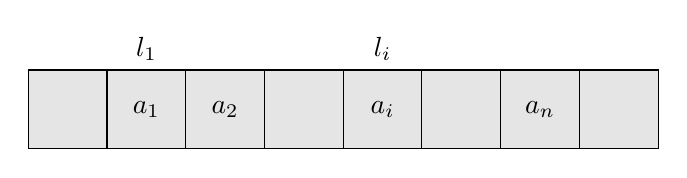
\begin{tikzpicture}
\foreach \i in {1,...,8}
\filldraw[fill=black!10] (\i-1,0)rectangle(\i,1);
\node [] at (0.5,0.5) {$\cd$};
\node [] at (1.5,0.5) {$a_1$}; \node [above] at (1.5,1) {$l_1$}; 
\node [] at (2.5,0.5) {$a_2$};
\node [] at (3.5,0.5) {$\cd$};
\node [] at (4.5,0.5) {$a_i$}; \node [above] at (4.5,1) {$l_i$}; 
\node [] at (5.5,0.5) {$\cd$};
\node [] at (6.5,0.5) {$a_n$};
\node [] at (7.5,0.5) {$\cd$};
\end{tikzpicture}
\caption{线性表的顺序存储}
\end{figure}
